\documentclass[11pt, twoside]{imsproc}

\usepackage{graphicx}
\usepackage{geometry}
\usepackage{booktabs}
\usepackage[colorlinks,citecolor=blue]{hyperref}
\setcounter{page}{1}
\geometry{left=2.5cm,right=2.5cm,top=3cm,bottom=3cm,headsep=1.1cm}
\footskip 0.7cm

%------------------------------------------------------------------------------------%
\newcommand*{\publname}{
\begin{tabular}{c}

\includegraphics[width=1.8cm]{UI-Logo.jpg}\\
\url{http://www.ui.ac.ir}
\vspace{0.2cm}
\end{tabular}
\hfill
\begin{tabular}{c}\toprule
\vspace{0.1cm}
\scriptsize \bfseries روش پژوهش و ارائه\\
\vspace{0.1cm}
\copyright{} \lr{1xxx} دانشگاه اصفهان \\ \bottomrule
\end{tabular}
\hfill
\begin{tabular}{c}

\includegraphics[width=2.2cm]{JMS-Logo.jpg}\\
\url{http://math-sci.ui.ac.ir}
\vspace{-0.2cm}
\end{tabular}
}
%------------------------------------------------------------------------------------%

\usepackage[para*]{manyfoot}
\SetFootnoteHook{\setLTR}
\DeclareNewFootnote[para]{A}
\usepackage{xepersian}
\makeatletter
\let\c@footnoteA\c@footnote
\makeatother
\let\LTRfootnote\footnoteA
\AtBeginDocument{\label{firstpage}}
\AtEndDocument{\label{lastpage}}
\settextfont[Scale=1.1]{XB Niloofar.ttf}
\setlatintextfont [Scale=0.9]{times new roman.ttf}
\linespread{1.35}
\newsavebox\uilogo
\newsavebox\nologo
\sbox\uilogo{
\includegraphics[width=0.8cm]{UI-Logo.pdf}}
\sbox\nologo{
\includegraphics[width=1cm]{JMS-Logo.jpg}}
\makeatletter
\def\seriesno#1{\gdef\@seriesno{#1}}
\def\issueno#1{\gdef\@issueno{#1}}
\def\publicationname#1{\gdef\@publicationname{#1}}
\def\ps@ijheadings{\ps@empty
  \def\@evenhead{%
   \parbox{\textwidth}{%
    \setTrue{runhead}%
    \normalfont\scriptsize
    \usebox\uilogo\hfill
    \def\thanks{\protect\thanks@warning}%
  \leftmark{}{}, \@publicationname/
    جلد x،
   % \@seriesno{}
    شماره x 
   % \@issueno
 (1xxx) \pageref{firstpage}--\pageref{lastpage}
    \hfill
   \usebox\nologo\vskip0pt
     \vskip-7pt
     \rule{\textwidth}{0.5pt}
      \vskip-12pt
        \rule{\textwidth}{0.5pt}
    }}
  \def\@oddhead{%
   \parbox{\textwidth}{%
    \setTrue{runhead}%
    \normalfont\scriptsize
    \usebox\uilogo\hfill
    \def\thanks{\protect\thanks@warning}%
    \rightmark{}{}, \@publicationname/
    جلد x،
    %\@seriesno{}
    شماره x 
    %\@issueno
 (1xxx) \pageref{firstpage}--\pageref{lastpage}
    \hfill
   \usebox\nologo\vskip0pt
     \vskip-6pt
     \rule{\textwidth}{0.5pt}
      \vskip-12pt
        \rule{\textwidth}{0.5pt}
    }}
   \def\@evenfoot{\normalfont\small\thepage
     \hfill \scriptsize{}\hfill}
    \def\@oddfoot{\normalfont\small\hfill\scriptsize{}\hfill\thepage}
 }%   
\def\enddoc@text{%
\ifx\@empty\@translators \else\@settranslators\fi
  \ifx\@empty\addresses \else\@setaddresses\fi}
  
\renewcommand*{\@makefnmark}{\hbox{\@textsuperscript{\normalfont\@thefnmark}}}
  \def\MFL@fnotepara#1#2#3{\let\@thefnmark\@empty
    \NCC@makefnmark{\latinfont #2}%
    \MFL@insert#1{\reset@font\footnotesize
      \ifx\@thefnmark\@empty \@tempswafalse \else
        \@tempswatrue
        \protected@edef\@currentlabel{\@thefnmark}%
      \fi
      \color@begingroup
        \if@tempswa
          \setbox\@tempboxa\hbox{\@makefnmark}%
          \ifMFL@paraindent
            \@tempdima.8em \advance\@tempdima-\wd\@tempboxa
            \ifdim \@tempdima<\z@ \@tempdima\z@ \fi
          \else
            \@tempdima\z@
          \fi
        \fi
        \setbox\@tempboxa\hbox{%
          \if@tempswa
            \hskip\@tempdima\unhbox\@tempboxa\nobreak
          \fi
          \ignorespaces\resetlatinfont#3\unskip\strut
          \ifMFL@split \penalty\m@ne\space \else
            \penalty-10 \hskip\footglue
          \fi
        }%
        \dp\@tempboxa\z@ \ht\@tempboxa\MFL@fudgefactor\wd\@tempboxa
        \box\@tempboxa
      \color@endgroup
    }%
  }
\long\def\@footnotetext#1{\insert\footins{%
   \if@RTL@footnote\@RTLtrue\else\@RTLfalse\fi%
    \reset@font\tiny
    \interlinepenalty\interfootnotelinepenalty
    \splittopskip\footnotesep
    \splitmaxdepth \dp\strutbox \floatingpenalty \@MM
    \hsize\columnwidth \@parboxrestore
    \protected@edef\@currentlabel{%
       \csname p@footnote\endcsname\@thefnmark
    }%
    \color@begingroup
      \@makefntext{%
        \rule\z@\footnotesep\ignorespaces\if@RTL@footnote#1\else\latinfont#1\fi\@finalstrut\strutbox}%
    \color@endgroup}}%
%\footdir@temp\footdir@my@ORG@xepersian@footnotetext\@footnotetext{\bidi@footdir@footnote}%
\makeatother
\pagestyle{ijheadings}
\seriesno{1}
\issueno{1}
\publicationname{}
\title{معماری کامپیوتر \lr{(Computer Architecture)}}
\author{
فاطمه علی‌ملکی، امیررضا جهانگیری، محمدحسین چهکندی، مهدی حق‌وردی و خدیجه نظری
}

\thanks{
عبارات و کلمات کليدي: {معماری کامپیوتر، واحد پردازش، \lr{x86}، \lr{arm}، \lr{qbit}}\\
دبیرتخصصی رابط: استاد دکتر فریا نصیری مفخم\\  
نوع مقاله: تکلیف کلاسی\\
تاریخ دریافت: 1400/9/14
\quad
تاریخ پذیرش: 1400/10/18 
}
\copyrightinfo{}{(دانشگاه اصفهان)}

\makeatletter
\def\ps@firstpage{\ps@plain
\def\@oddfoot{\normalfont\small\hfil\thepage\hfil
\global\topskip\normaltopskip}%
\let\@evenfoot\@oddfoot
\def\@oddhead{\@serieslogo\hss}%
\let\@evenhead\@oddhead % in case an article starts on a left-hand page
}
%%%%%%%%%%%%%%%%%
\settextfont[Scale=1.1]{Yas}
%%%%%%%%%%%%%%%%%%%%%%%
\makeatother
\begin{document}
\begin{abstract}
در این مقاله، به بررسی معماری کامپیوتر، روند توسعه‌ی آن، انواع معماری کامپیوتر و پیشرفت‌های آن می‌پردازیم.
\end{abstract}
\maketitle
\section{مقدمه}

\section{معماری کامپیوتر - دیروز تا امروز}
\vskip 0.4 true cm

در دنیایی که ما امروزه می‌شناسیم رایانه‌ها برای اهداف زیاد و توسط افراد زیادی استفاده می‌شوند. آنها قادرند چیزهای جذابی را به نمایش بگذارند که ذهن مارا متحیر میکند. اتفاقی که زمانی غیر قابل تصور بود برای جامعه ما مرسوم است.

تکنولوژی معماری کامپیوتر در طول سالیان متمادی تکامل یافته است. تغییرات در معماری کامپیوتری عمدتاً به دلیل پیشرفت‌های تکنولوژی ساخت قطعات الکترونیکی، نیاز‌های کاربران و پیشرفت علوم رخ داده است. در ادامه به خلاصه‌ای از تکامل معماری کامپیوتر از زمان ظهور اولین کامپیوترها تا به امروز می‌پردازیم. 

\begin{enumerate}
\item نسل اول کامپیوترها

در سال ۱۹۳۷، اولین کامپیوتر با استفاده از لامپ‌های خلاء توسط پروفسور ایکن اختراع شد. در سال ۱۹۴۷، دانشگاه پنسیلوانیا کامپیوتری به نام \lr{ENIAC} را طراحی کرد که از مبنای دودویی برای نمایش اطلاعات استفاده می‌کرد.\footnote{مشهورترین نمونه از این دوره می‌باشد} در این دوره، کامپیوترها از لامپ‌های خلاء و رله‌ها برای اجرای عملیات استفاده می‌کردند.
معماری کامپیوترهای این دوره معمولاً به صورت برداری \lr{(Von Neumann)} بود که شامل واحدهای حافظه، واحد پردازش، واحد کنترل و واحد ورودی/خروجی می‌شد.

\item نسل دوم کامپیوترها

در دهه ۱۹۵۰، ترانزیستورها به جای لامپ‌های خلاء در کامپیوترها استفاده شدند. این باعث کاهش حجم و افزایش سرعت کامپیوترها شد. در این دوره، کامپیوترهای دیجیتال شروع به ظهور کردند و از معماری فرمال برای طراحی استفاده می‌شد. این دوره شاهد ظهور کامپیوترهای دیجیتال و کامپیوترهای مینی‌کامپیوتر بود.

\item نسل سوم کامپیوترها

در دهه ۱۹۶۰، مدارهای مجتمع\LTRfootnote{\lr{IC}} جایگزین ترانزیستورها شدند. استفاده از مدارهای مجتمع باعث افزایش قابلیت پیچیدگی و کارایی کامپیوترها شد. به این معنی که تعداد بیشتری ترانزیستور و قطعه الکترونیکی را در یک تراشه کوچک‌تر قرار دادند. این امر به کامپیوترها امکان انجام عملیات پیچیده‌تر و سریع‌تر را می‌داد. به طور خلاصه، مدارهای مجتمع به کامپیوترها امکانات بیشتری را بخشیدند و آن‌ها را کارآمدتر می‌ساختند. در این دوره، معماری مینی‌کامپیوترها و سوپرکامپیوترها توسعه یافت. در این دوره، مدارهای مجتمع بزرگتر و پیچیده‌تری استفاده شدند. کامپیوترهای این دوره از معماری مجموعه دستورات\LTRfootnote{\lr{Instruction Set Architecture}} استفاده می‌کردند. معماری کامپیوتر \lr{IBM/360} از معماری‌های مشهور این دوره است.

\item نسل چهارم کامپیوترها

در دهه ۱۹۷۰، ریزپردازنده‌ها\LTRfootnote{\lr{Microcontroller}} به جای مدارهای مجتمع استفاده شدند. این باعث افزایش قابلیت انعطاف‌پذیری و کاهش هزینه ساخت کامپیوترها شد. در این دوره، معماری کامپیوترهای شخصی و کامپیوترهای قابل حمل توسعه یافت 

\item نسل پنجم کامپیوترها

در دوره نسل پنجم کامپیوترها، که در دهه 1980 آغاز شد، تحولات مهمی در معماری کامپیوتر رخ داد. در این دوره، دو نوع کامپیوتر مهم به وجود آمدند: کامپیوترهای موازی و کامپیوترهای برداری. کامپیوترهای موازی قدرت پردازش را با استفاده از چندین واحد پردازشگر به صورت همزمان افزایش می‌دادند. این کامپیوترها قابلیت انجام همزمان و همروند بسیاری از عملیات‌ها را داشتند و برای برنامه‌هایی که نیاز به پردازش موازی داشتند، بسیار مناسب بودند.
کامپیوترهای برداری قدرت پردازش را با استفاده از پردازشگرهای برداری بهبود می‌بخشیدند. این پردازشگرها برای عملیات‌های مربوط به بردارها و ماتریس‌ها بهینه شده بودند و برای برنامه‌های علمی و مهندسی که با داده‌های برداری سر و کار داشتند، مناسب بودند.
در این دوره، استفاده از مدارهای مجتمع فوق بزرگ\LTRfootnote{\lr{VLSI}} و مدارهای مجتمع فوق فوق بزرگ\LTRfootnote{\lr{ULSI}} نیز رایج شد. این تکنولوژی‌ها به طراحی و ساخت مدارهای بسیار پیچیده و کوچکتر از نسل‌های قبلی کمک کردند و باعث افزایش کارایی و قدرت پردازش کامپیوترها شدند.
در این دوره، شاهد ظهور کامپیوترهای جدیدی نیز بودیم که از جمله آن‌ها می‌توان به کامپیوترهای شخصی\LTRfootnote{\lr{Personal Computers}} و سیستم‌های توزیع شده\LTRfootnote{\lr{Distributed Systems}} اشاره کرد. کامپیوترهای شخصی با عملکرد مناسب و هزینه کم، به کاربران خانگی و کسب و کارها وارد شدند و سیستم‌های توزیع شده با استفاده از شبکه‌های کامپیوتری، امکان ارتباط و همکاری بین کامپیوترها را فراهم می‌کردند.   

\end{enumerate}

%------------------------------------------------------------------------------------------------
%نوشتن بیوگرافی نویسندگان الزامی می باشد.

\bigskip
\bigskip 

\noindent \rule{.4\linewidth}{0.8pt}\\
\noindent\footnotesize{\bfseries نام و نام خانوادگی نویسنده اول} \\
\footnotesize{اصفهان، خيابان هزار جريب، دانشگاه اصفهان، گروه ریاضی } \\
abc@yahoo.com\\\\
\begin{tabular}{p{2 cm} p{14 cm} }
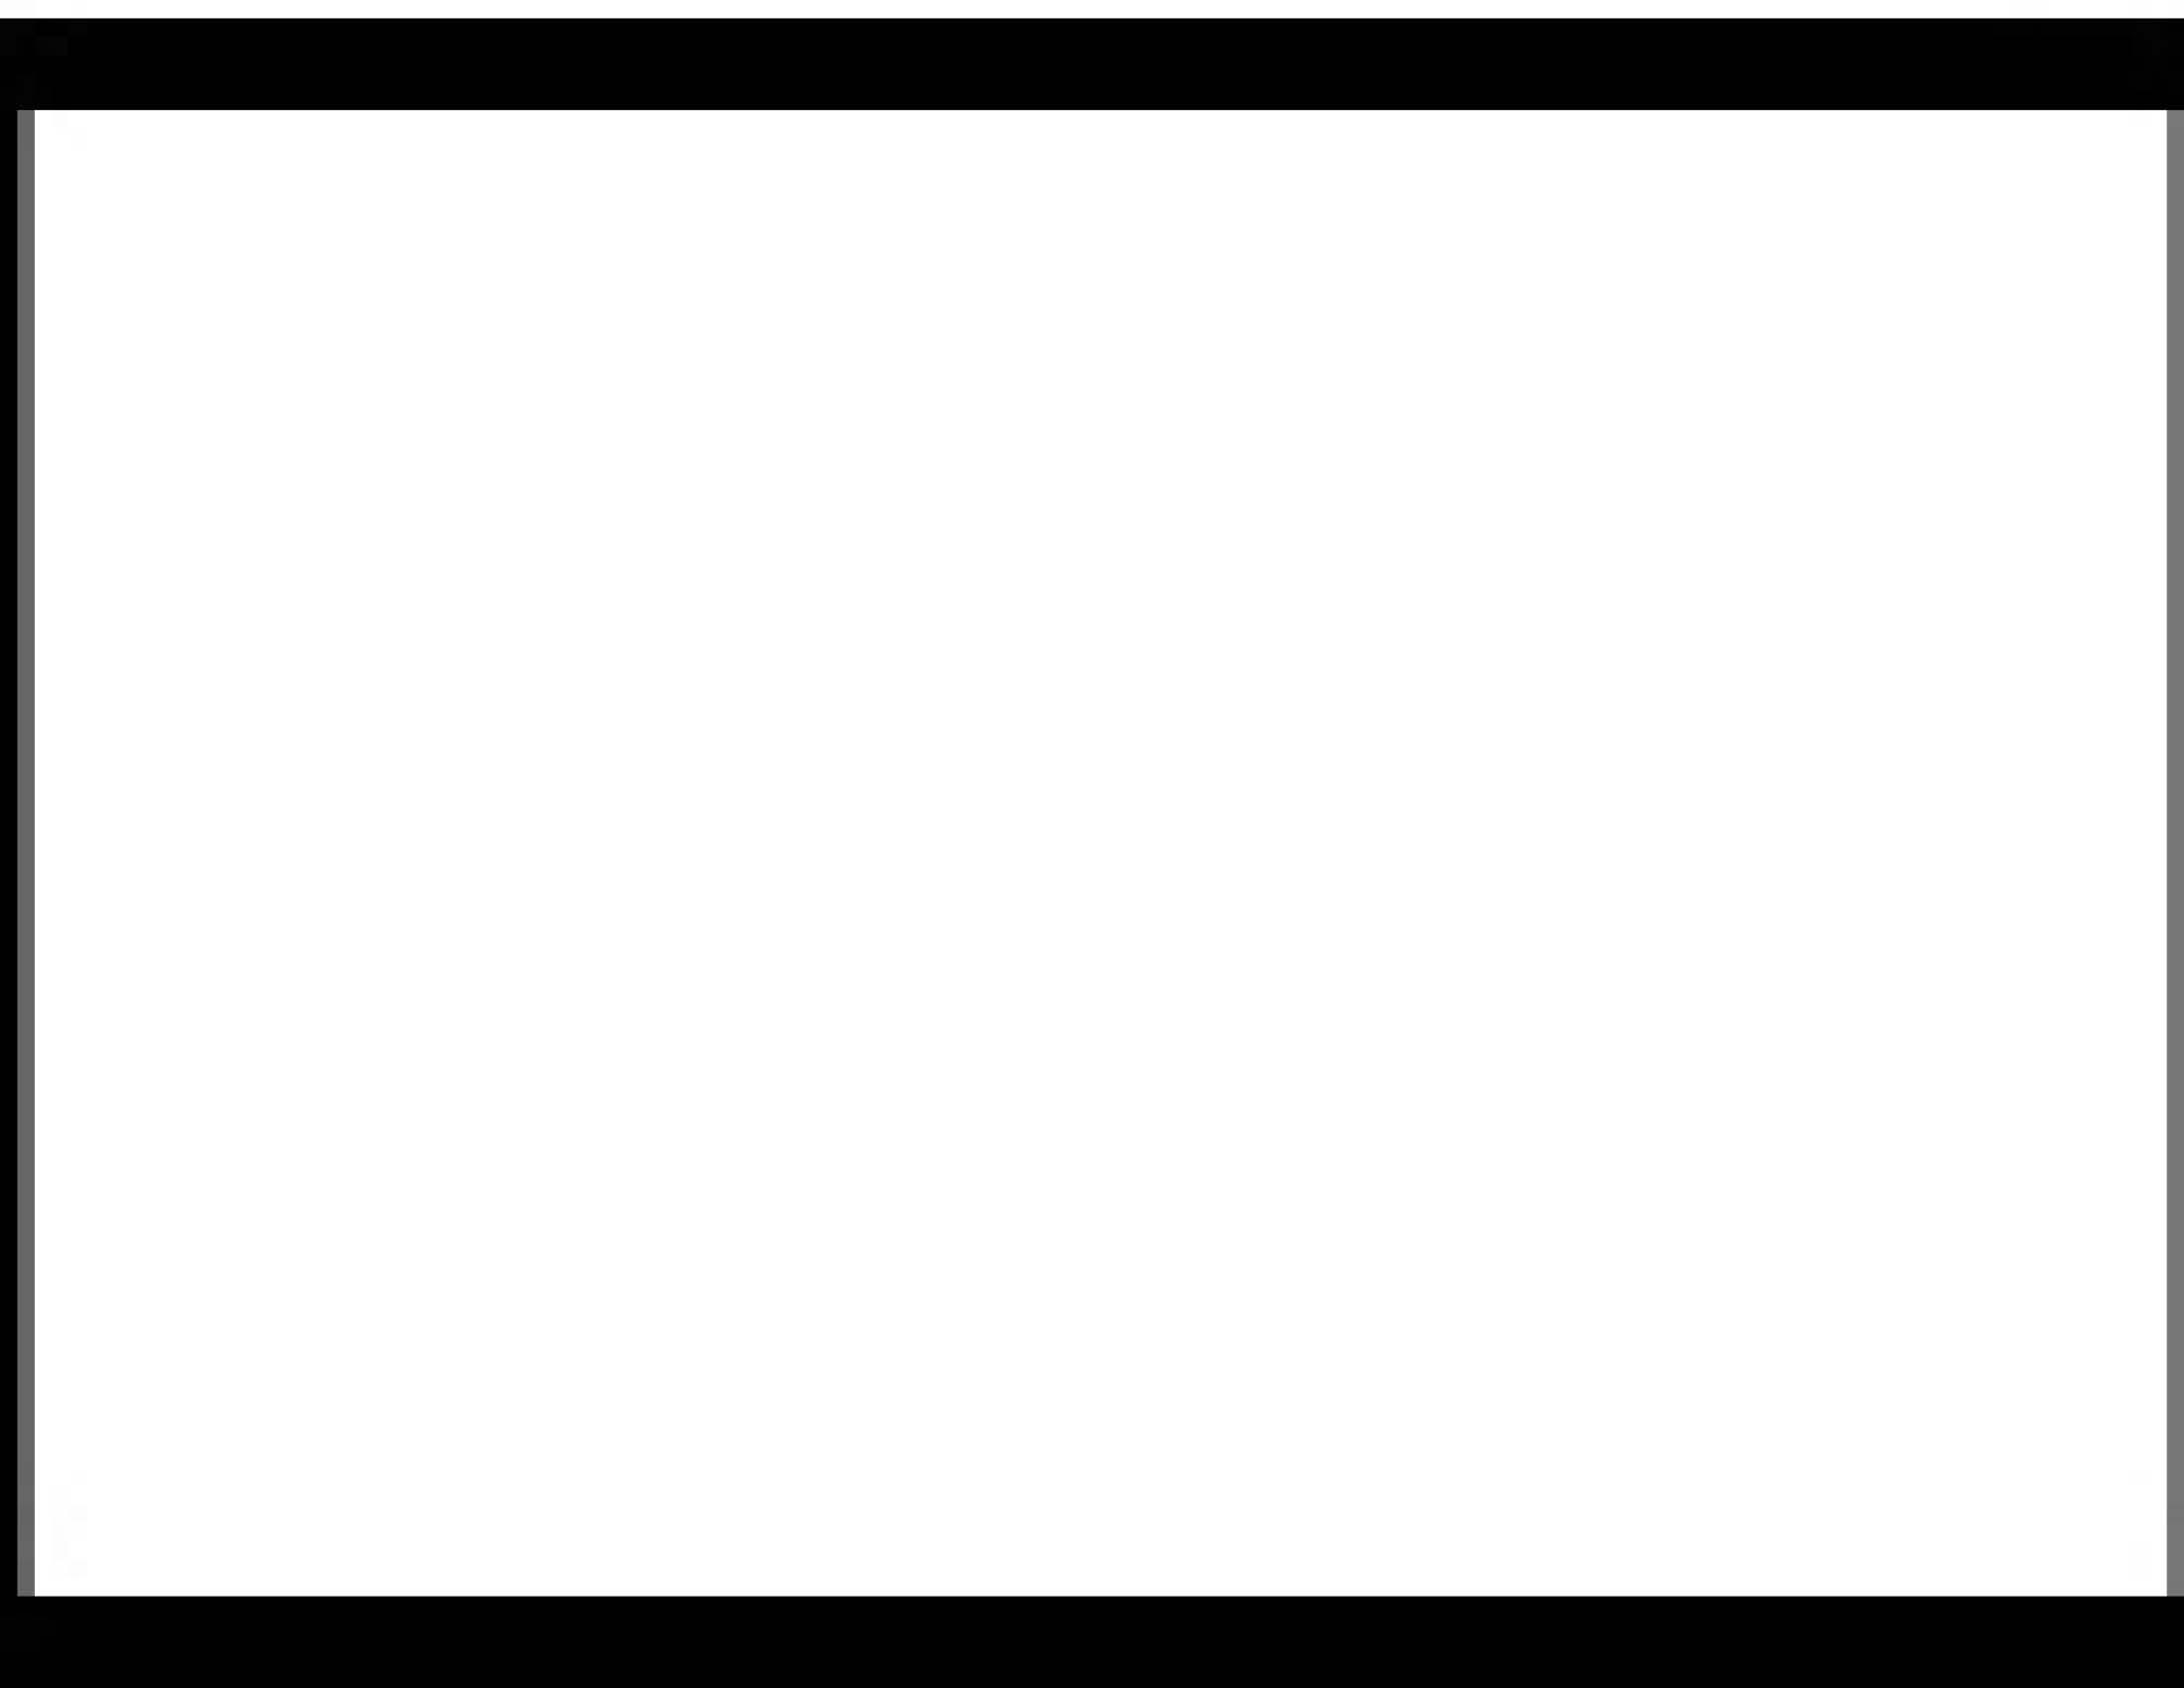
\includegraphics[width=20mm]{Image1} 
&\vspace{-1.5cm}
\footnotesize

نویسنده اول (یا مترجم) متولد مهرماه ماه 1361 در شهر اصفهان است. وی در سال 1380 وارد مقطع كارشناسی رشته رياضی محض دانشگاه اصفهان شد و در سال 1385 وارد مقطع كارشناسی ارشد رشته رياضی محض شد.\\
\end{tabular}\\\\
\noindent\footnotesize{\bfseries نام و نام خانوادگی نویسنده دوم } \\
\footnotesize{تهران، دانشگاه تهران، گروه ریاضی } \\
 def@gmail.com\\\\
\begin{tabular}{p{2 cm} p{14 cm} }
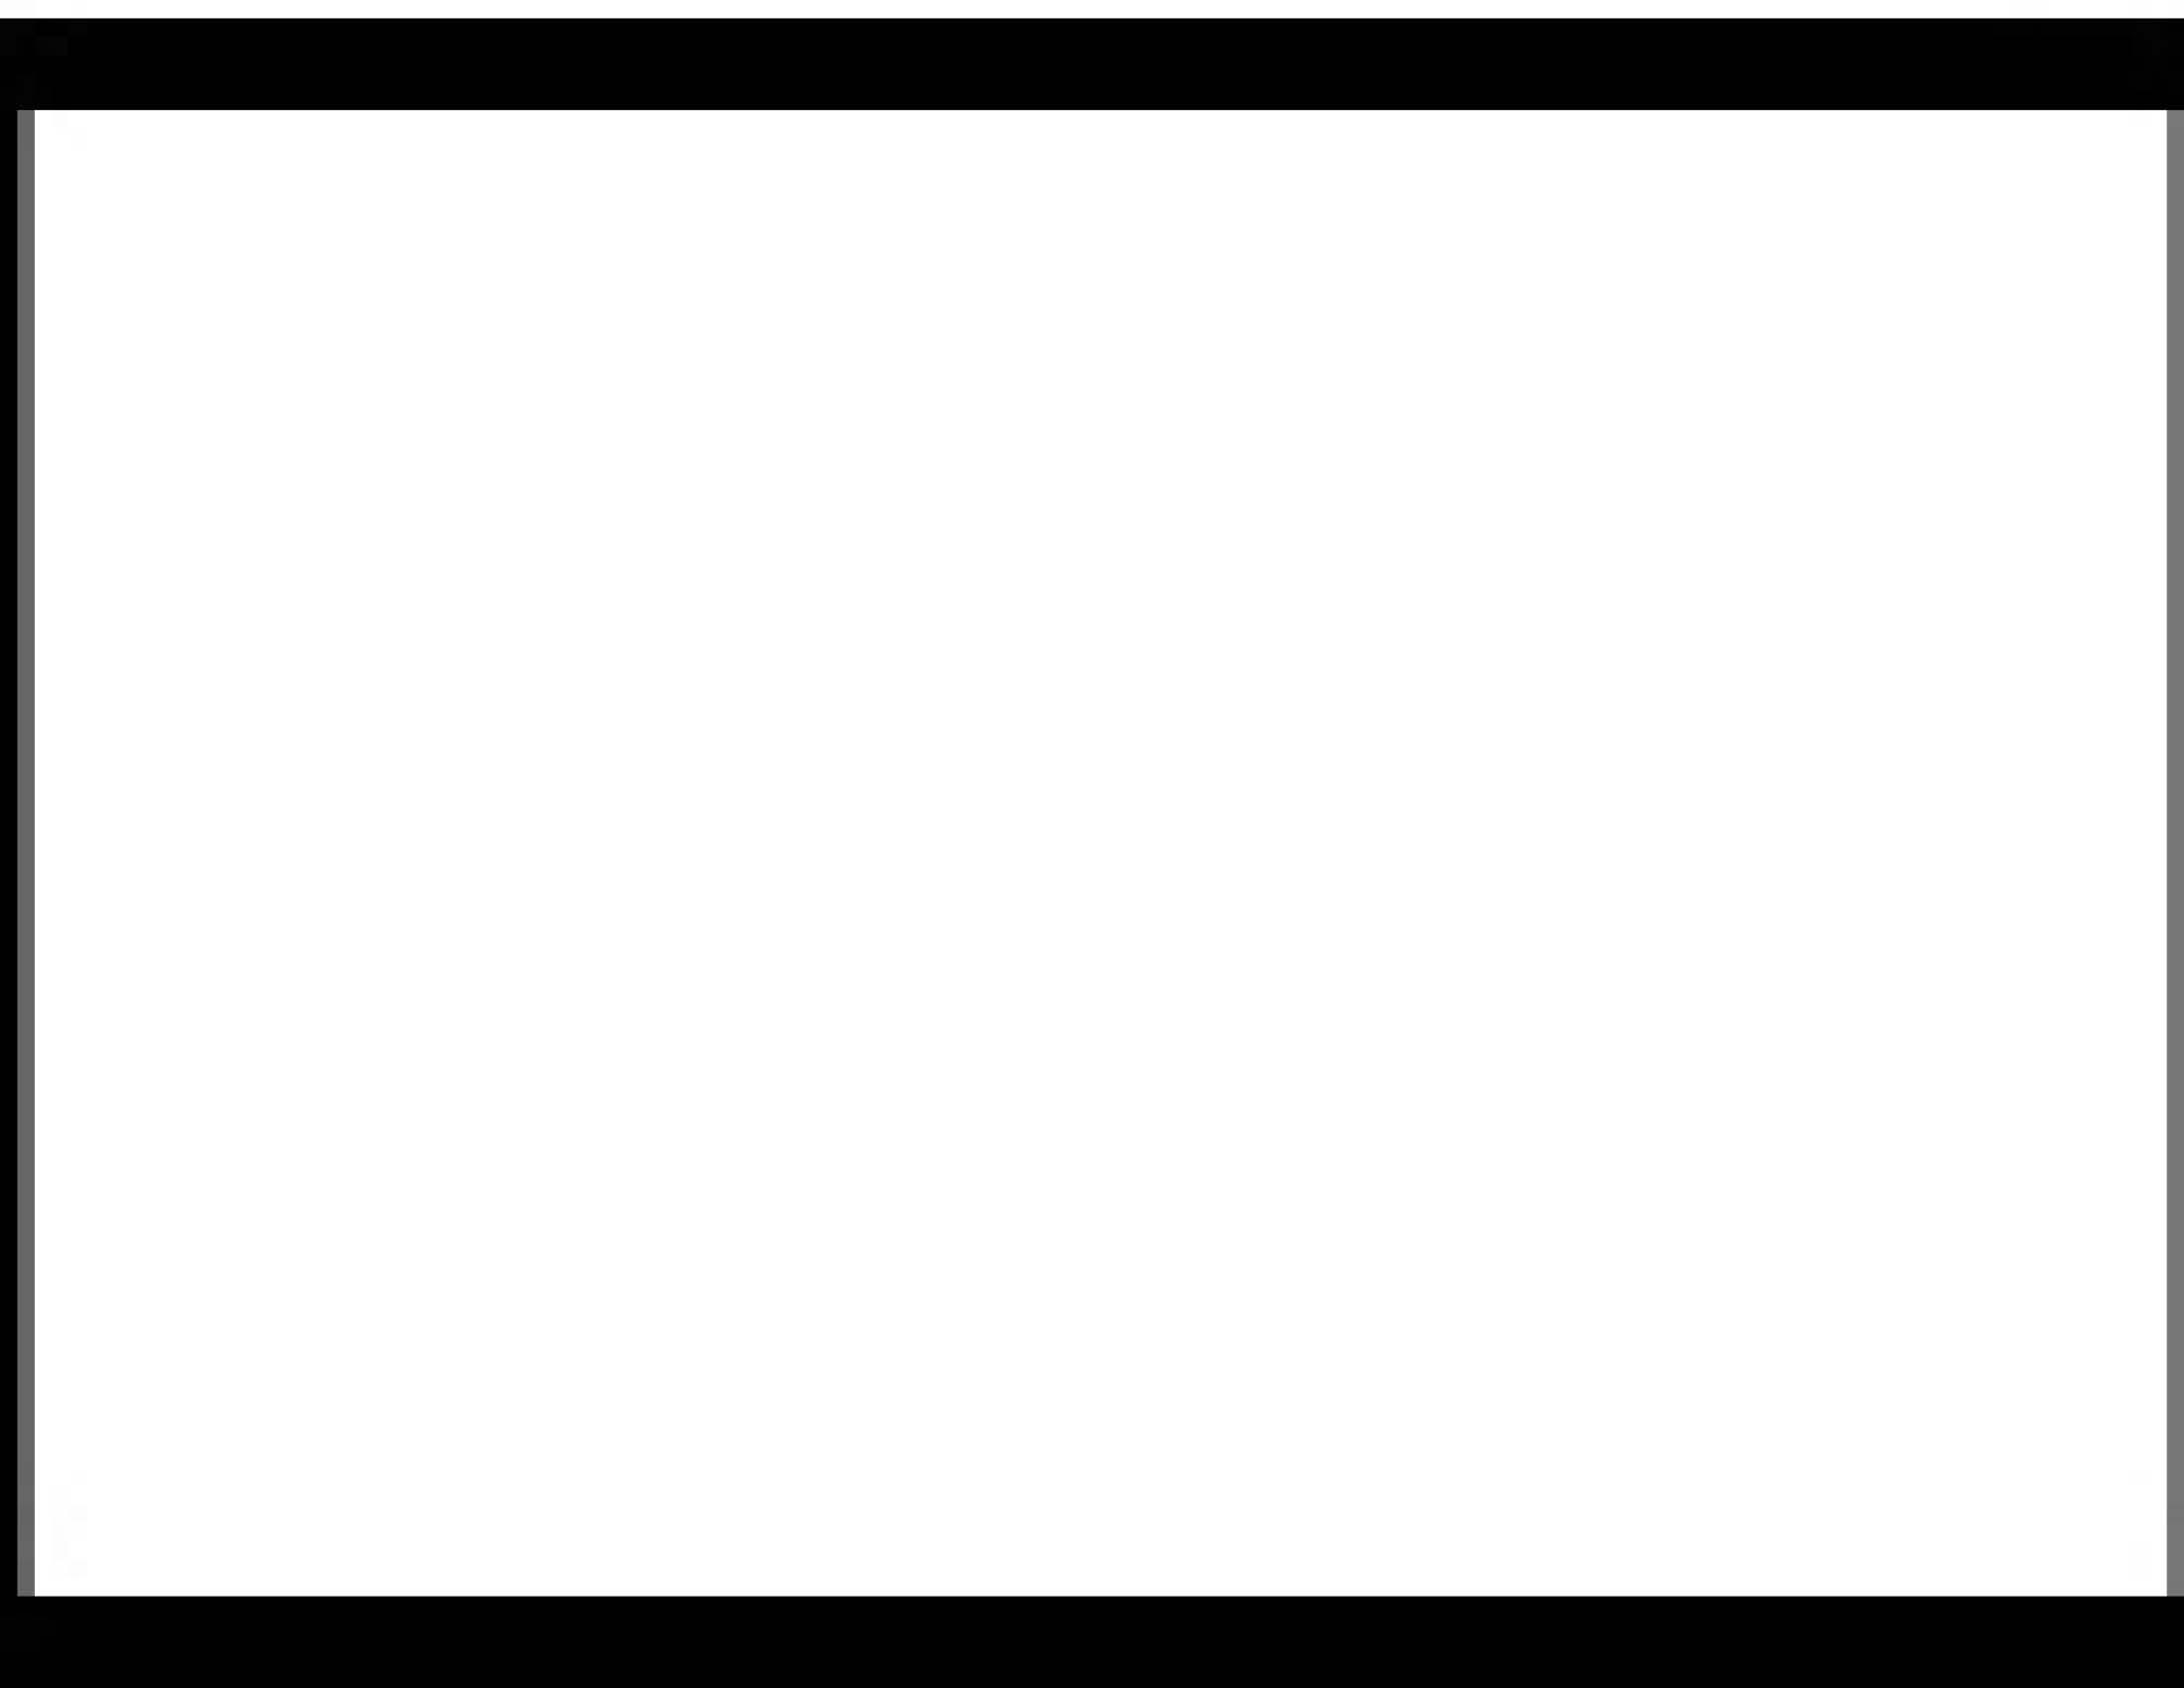
\includegraphics[width=20mm]{Image2} 
&\vspace{-1.5cm}
\footnotesize

نویسنده دوم متولد مرداد ماه 1368 در شهر تهران است. وی در سال 1386 وارد مقطع كارشناسی رشته رياضی كاربردی دانشگاه تهران شد و در سال 1390  وارد مقطع كارشناسی ارشد رشته رياضی كاربردی شد.
\end{tabular}
\end{document}